
%Si el proyecto es continuación de otro previamente financiado, individual o coordinado, deben indicarse con claridad los objetivos y los resultados ya alcanzados de manera que sea posible evaluar el avance real que se propone en el nuevo proyecto. Si el proyecto aborda un tema nuevo, deben indicarse los antecedentes y contribuciones previas de los equipos de investigación que justifiquen su capacidad para llevarlo a cabo.
%

This research project is the continuation of the CONSOLIDER-INGENIO project CUP (2010-2014), and the SEIDI project FIS2012-37947-C04 (2012-2014). 

The initial phase of the project (called the DEMO phase), included a learning period (2010-2011), needed to acquire the very innovative technology the detector is based on, and to equip state-of-the-art laboratories at IFIC and other participating institutions. 
During 2011 and 2012, the collaboration selected the technology to be implemented and a Technical Design Report\footcite{Alvarez:2012haa} was published in 2012. This phase of the project culminated  with the construction, commissioning and operation of the NEXT-DEMO prototype located at IFIC, and the NEXT-DBDM prototype operating at LBNL. During 2012 and 2013, the results of the prototypes were analysed and published, showing the excellent performance (energy resolution, electron reconstruction) of the apparatus, as well as the robustness of the EL technology\footcite{Alvarez:2012hh, Alvarez:2012nd, Alvarez:2012hu,Alvarez:2013gxa,Lorca:2014sra}. 

\subsubsection*{NEXT prototypes}

\begin{figure}
\centering
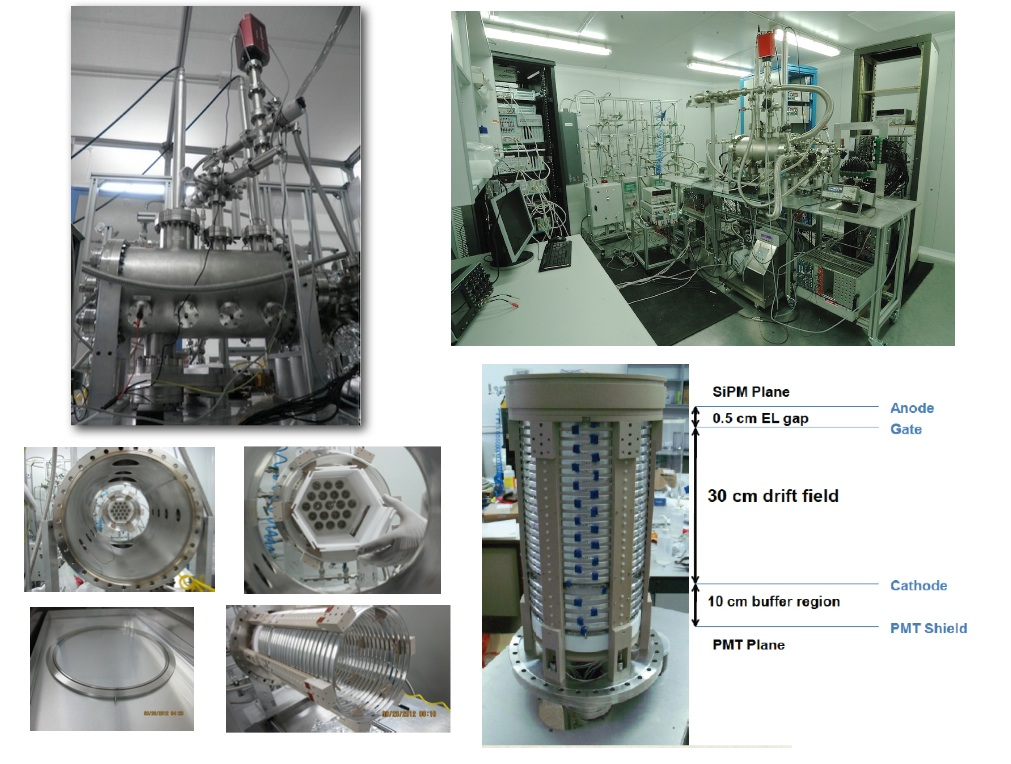
\includegraphics[width=0.8\textwidth]{img/DemoSetup2.jpg}
\caption{\small The NEXT-DEMO prototype. Top-left: the pressure vessel, showing the HVFT and the mass spectrometer; bottom-left: an expanded view of the detector; (c) Teflon light tube; (d) energy plane, made of pressure resistant Hamamatsu R7378A PMTs; (e) field cage; (f) tracking plane equipped with 300 Hamamatsu MPPCs; top-right: the full setup at IFIC; bottom right: the field cage.} \label{fig.DEMO}
\end{figure}
%%%%%%%%%%

NEXT-DEMO, shown in figure \ref{fig.DEMO}, is as a large-scale prototype of NEXT-100. The pressure vessel has a length of 60 cm and a diameter of 30 cm. The vessel can withstand a pressure of up to 15 bar and hosts typically 1-2 kg of xenon. NEXT-DEMO is  equipped with an energy plane made of 19 Hamamatsu R7378A PMTs and a tracking plane made of 256 Hamamatsu SiPMs. 

The detector has been operating successfully for more than two years and has demonstrated: (a) very good operational stability, with no leaks and very few sparks; (b) good energy resolution ; (c) track reconstruction with PMTs and with SiPMs coated with TPB; (d) excellent electron drift lifetime, of the order of 20 ms.Its construction, commissioning and operation has been instrumental in the development of the required knowledge to design and build the NEXT detector.

The NEXT-DBDM prototype is a smaller chamber, with only 8 cm drift, but an aspect ratio (ratio diameter to length) similar to that of NEXT-100. The device has been used to perform detailed energy resolution studies. NEXT-DBDM achieves a resolution of 1\% FWHM at 660 keV and 15 bar, which extrapolates to 0.5\% at \Qbb.

\subsubsection*{Topological signature}

%%%%%
\begin{figure}
\centering
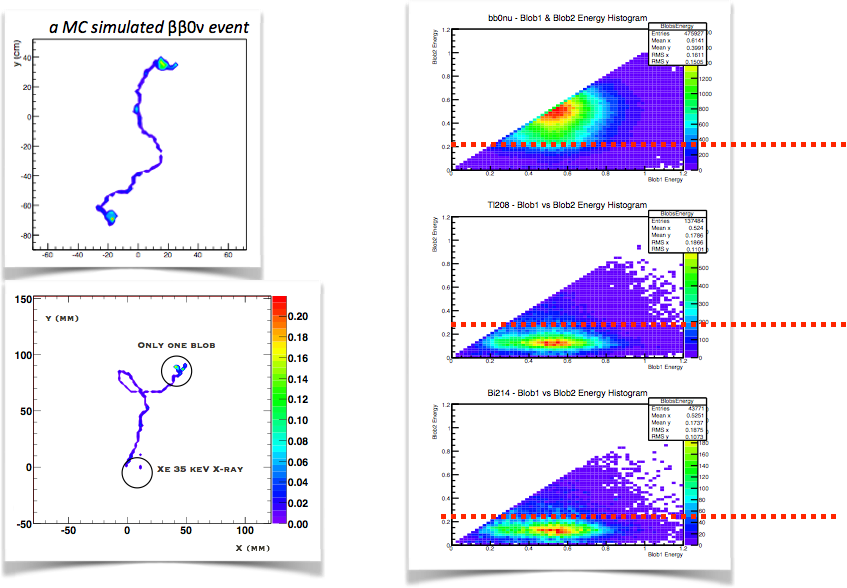
\includegraphics[width=0.9\textwidth]{img/Topology.png}
\caption{\small NEXT has a topological signature, not available in most \bbonu\ detectors. The panel shows the reconstruction of a Monte Carlo signal (topleft) and background (bottomleft) event. The signal has two electrons (two blobs). The background has only one electron (one blob) and the associated emission of a 35 keV X-ray. The color codes energy deposition in the TPC. An scatter plot of the energy of the two blobs shows a clear separation between signal and background regions.}\label{fig.ETRK2}
\end{figure}
%%%%%

%%%%%%
%\begin{figure}
%\centering
%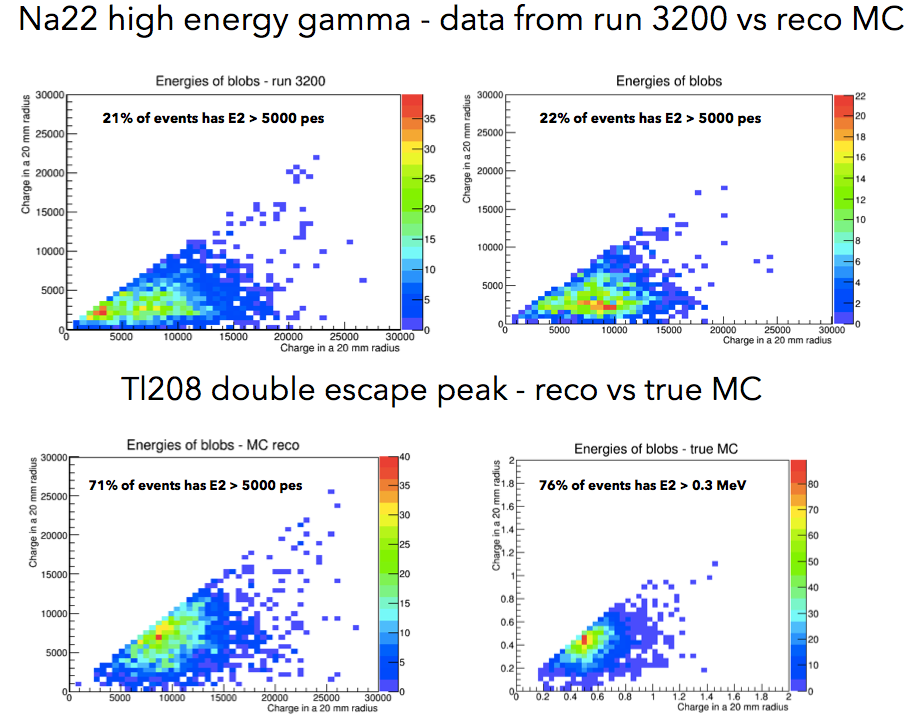
\includegraphics[width=0.9\textwidth]{img/ElectronsDataMC.png}
%\caption{\small A comparison between data (left) and Monte Carlo (right) for electrons of different energies recorded in the DEMO chambers, showing the very good agreement between both data sets and therefore the robustness of the topological signal, unique of the NEXT experiment.}\label{fig.ETRK3}
%\end{figure}
%

Double beta decay events leave a distinctive topological signature in HPXe: a continuous track with larger energy depositions (\emph{blobs}) at both ends due to the Bragg-like peaks in the d$E$/d$x$ of the stopping electrons (figure \ref{fig.ETRK2}, topleft). In contrast, background electrons are produced by Compton or photoelectric interactions, and are characterised by a single blob and, often, by a satellite cluster corresponding to the emission of $\sim30$-keV fluorescence x-rays by xenon (figure \ref{fig.ETRK2}, bottomleft).
Reconstruction of this topology using the tracking plane provides a powerful means of background rejection, as can be observed in the figure. In our TDR we chose a conservative cut to separate double--blob from single--blob events which provided a suppression factor of 20 for the background while keeping 80\% of the signal.  DEMO has reconstructed single electrons from \NA\ and \CS\ sources, as well as double electrons from the double escape peak of \TL\, demonstrating the robustness of the topological signal. 

%
%Figure \ref{fig.ETRK3} shows a comparison between data and Monte Carlo for electrons interacting in the DEMO detector. Two radioactive sources were used: Na-22, producing single electrons of 511 keV, and Tl-208, whose double escape peak produced {\em double electrons}, at the energy of 1.6 MeV. Both data sets allow us to ``mimic'' signal and background and thus have a robust assessment of the performance of the topological signal comparing the Monte Carlo simulation and the actual results obtained with DEMO. The agreement between both data sets is very good, revealing the robustness of the topological signal. 

\subsubsection*{Energy resolution}

%%%%%
\begin{figure}
\centering
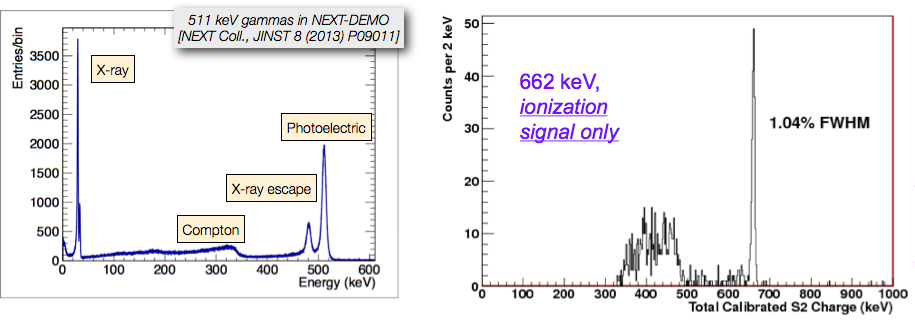
\includegraphics[width=0.9\textwidth]{img/EResolution.png}
\caption{\small Left: the full energy spectrum measured for electrons of 511 keV in the DEMO detector. Right the spectrum near the photoelectric peak for 662 keV electrons in NEXT-DBDM. The resolution at 662 keV is 1\% FWHM (0.5\% FWHM at \Qbb). The resolution extrapolated from 511 keV is 0.7\%.}\label{fig.ERES}. 
\end{figure}
%%%%

Figure \ref{fig.ERES} shows the resolution obtained with the NEXT-DBDM apparatus. A resolution of 1\% FWHM with 
662 keV photons, has been measured, which extrapolates to 0.5\% FWHM at \Qbb. This result is not far from the expected limit obtained adding in quadrature the different factors that contribute to the resolution (Fano factor, photoelectron statistics and electronic noise). The resolution measured in NEXT-DEMO extrapolates to 0.7\% FWHM. The difference between both prototypes is due to better photoelectron statistics and aspect ratio in DBDM. The results, are, in any case, better than the target of 1\% FWHM described in the TDR.

The status of the NEXT experiment and the results achieved by the prototypes have been described in a recent
paper \footcite{Gomez-Cadenas:2013lta}.

